\hypertarget{stm32f4xx__hal__flash_8c}{}\section{Dokumentacja pliku S\+T\+M/\+W\+D\+S\+\_\+\+Kosc\+\_\+\+Linux/\+Drivers/\+S\+T\+M32\+F4xx\+\_\+\+H\+A\+L\+\_\+\+Driver/\+Src/stm32f4xx\+\_\+hal\+\_\+flash.c}
\label{stm32f4xx__hal__flash_8c}\index{S\+T\+M/\+W\+D\+S\+\_\+\+Kosc\+\_\+\+Linux/\+Drivers/\+S\+T\+M32\+F4xx\+\_\+\+H\+A\+L\+\_\+\+Driver/\+Src/stm32f4xx\+\_\+hal\+\_\+flash.\+c@{S\+T\+M/\+W\+D\+S\+\_\+\+Kosc\+\_\+\+Linux/\+Drivers/\+S\+T\+M32\+F4xx\+\_\+\+H\+A\+L\+\_\+\+Driver/\+Src/stm32f4xx\+\_\+hal\+\_\+flash.\+c}}


F\+L\+A\+SH H\+AL module driver. This file provides firmware functions to manage the following functionalities of the internal F\+L\+A\+SH memory\+:  


{\ttfamily \#include \char`\"{}stm32f4xx\+\_\+hal.\+h\char`\"{}}\newline
Wykres zależności załączania dla stm32f4xx\+\_\+hal\+\_\+flash.\+c\+:\nopagebreak
\begin{figure}[H]
\begin{center}
\leavevmode
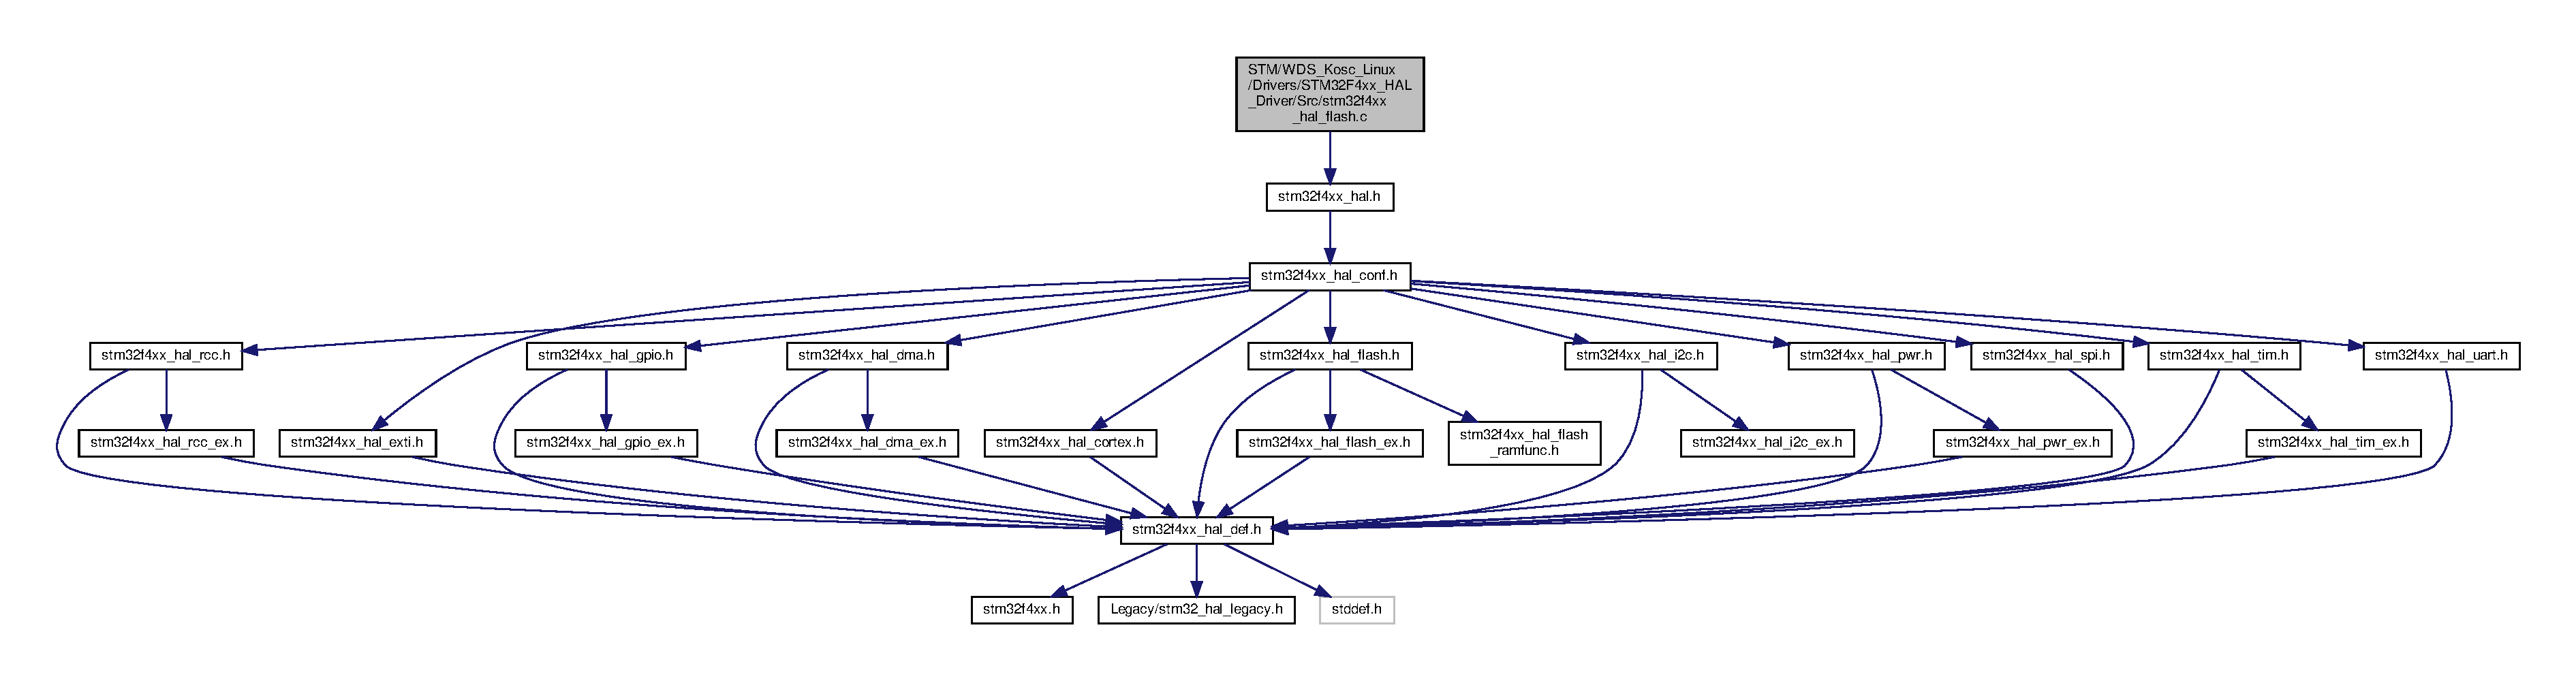
\includegraphics[width=350pt]{stm32f4xx__hal__flash_8c__incl}
\end{center}
\end{figure}


\subsection{Opis szczegółowy}
F\+L\+A\+SH H\+AL module driver. This file provides firmware functions to manage the following functionalities of the internal F\+L\+A\+SH memory\+: 

\begin{DoxyAuthor}{Autor}
M\+CD Application Team
\begin{DoxyItemize}
\item Program operations functions
\item Memory Control functions
\item Peripheral Errors functions
\end{DoxyItemize}
\end{DoxyAuthor}
\begin{DoxyVerb}==============================================================================
                      ##### FLASH peripheral features #####
==============================================================================
         
[..] The Flash memory interface manages CPU AHB I-Code and D-Code accesses 
     to the Flash memory. It implements the erase and program Flash memory operations 
     and the read and write protection mechanisms.
    
[..] The Flash memory interface accelerates code execution with a system of instruction
     prefetch and cache lines. 

[..] The FLASH main features are:
    (+) Flash memory read operations
    (+) Flash memory program/erase operations
    (+) Read / write protections
    (+) Prefetch on I-Code
    (+) 64 cache lines of 128 bits on I-Code
    (+) 8 cache lines of 128 bits on D-Code
    
    
                   ##### How to use this driver #####
==============================================================================
  [..]                             
    This driver provides functions and macros to configure and program the FLASH 
    memory of all STM32F4xx devices.
  
    (#) FLASH Memory IO Programming functions: 
         (++) Lock and Unlock the FLASH interface using HAL_FLASH_Unlock() and 
              HAL_FLASH_Lock() functions
         (++) Program functions: byte, half word, word and double word
         (++) There Two modes of programming :
          (+++) Polling mode using HAL_FLASH_Program() function
          (+++) Interrupt mode using HAL_FLASH_Program_IT() function
  
    (#) Interrupts and flags management functions : 
         (++) Handle FLASH interrupts by calling HAL_FLASH_IRQHandler()
         (++) Wait for last FLASH operation according to its status
         (++) Get error flag status by calling HAL_SetErrorCode()          

  [..] 
    In addition to these functions, this driver includes a set of macros allowing
    to handle the following operations:
     (+) Set the latency
     (+) Enable/Disable the prefetch buffer
     (+) Enable/Disable the Instruction cache and the Data cache
     (+) Reset the Instruction cache and the Data cache
     (+) Enable/Disable the FLASH interrupts
     (+) Monitor the FLASH flags status\end{DoxyVerb}


\begin{DoxyAttention}{Uwaga}

\end{DoxyAttention}
\subsubsection*{\begin{center}\copyright{} Copyright (c) 2017 S\+T\+Microelectronics. All rights reserved.\end{center} }

This software component is licensed by ST under B\+SD 3-\/\+Clause license, the \char`\"{}\+License\char`\"{}; You may not use this file except in compliance with the License. You may obtain a copy of the License at\+: opensource.\+org/licenses/\+B\+S\+D-\/3-\/\+Clause 